\documentclass[a4paper]{report}
\input{../../Templates/preamble.tex}
%PER CAMBIARE I MARGINI
\usepackage[margin=4cm]{geometry}

%----------- Setup stilistico ----------------
\definecolor{DarkRed}{HTML}{B6321C}
\hypersetup{
    colorlinks=true,
    linkcolor=DarkRed,
    filecolor=blue,
    citecolor = black,
    urlcolor=cyan,
}
\renewcommand\thefootnote{\textcolor{blue}{\arabic{footnote}}}
% ============================================


%---------- Comandi specifici ----------------


%--------- Comandi dattilografici ------------
\NewDocumentCommand{\ddb}{O{}mmm}{
    {\left.\frac{d^{#1}{#3}}{d{#2}^{#1}}\right|_{#4}}
}
\NewDocumentCommand{\ppb}{O{}mmm}{
    {\left.\frac{\partial^{#1}{#3}}{\partial{#2}^{#1}}\right|_{#4}}
}

% ============================================
\title{Fisica 3\\
\large Corso del prof. Sozzi Marco}

\author{Francesco Sorce}
\date{Università di Pisa\\
Dipartimento di Matematica\\
A.A. 2023/24}

\begin{document}
\maketitle

%\newpage
\tableofcontents
\newpage


\part{Termodinamica}
\chapter{Introduzione e Temperatura empirica}
\noindent
La termodinamica \`e lo studio di sistemi dal punto di vista macroscopico.\\
Le massime fondamentali della termodinamica sono
\begin{itemize}
\item L'energia dell'universo \`e costante
\item L'entropia dell'universo tende ad aumentare.
\end{itemize}

\section{Prime definizioni}
\begin{definition}[Sistema termodinamico]
Un \textbf{sistema termodinamico} \`e un sistema omogeneo composto da ``molti" elementi.\\
Lo \textbf{stato} di un sistema termodinamico \`e univocamente determinato da un numero contenuto di parametri\footnote{Per esempio temperatura, pressione o volume.} detti \textbf{funzioni di stato}.\\
Il numero di funzioni di stato necessarie per specificare lo stato \`e detto \textbf{numero di gradi di libert\`a}.
\end{definition}

\begin{remark}
Le funzioni di stato di un sistema non dipendono da come esso \`e venuto ad esistere; se due procedimenti portano da un particolare stato ad un altro, le differenze nelle funzioni di stato dipendono univocamente dallo stato iniziale e quello finale.
\end{remark}

\begin{remark}[Sistema ambiente]
Spesso torna comodo considerare una coppia di sistemi, uno detto semplicemente sistema e l'altro \textbf{ambiente}.
\end{remark}

\begin{definition}[Variabili estensive e intensive]
Dato un sistema termodinamico, delle variabili ad esso inerenti si dicono \textbf{estensive} se sono proporzionali alla quantit\`a di materia contenuta nel sistema e \textbf{intensive} altrimenti.
\end{definition}

\begin{example}
Il volume e l'energia sono grandezze estensive mentre la pressione e la temperatura sono intensive.
\end{example}

\begin{remark}
Il lavoro meccanico \`e dato da $W=\int \vec F\cdot \vec{d\ell}$. \`E un fatto generale che il lavoro ha la forma
\[\int(\text{intensiva})d(\text{estensiva}).\]
\end{remark}

\begin{definition}[Sistemi isolati, chiusi e aperti]
Un sistema termodinamico si dice 
\begin{itemize}
\item \textbf{isolato} se non ammette scambio con l'ambiente,
\item \textbf{chiuso} se non ammette scambio di materia con l'ambiente,
\item \textbf{aperto} se ammette scambi con l'ambiente.
\end{itemize}
\end{definition}

Per considerare pi\`u sistemi termodinamici dobbiamo considerarli come separati da una \textit{parete}.

\begin{definition}[Tipi di parete]
Una parete tra due sistemi \`e
\begin{itemize}
\item \textbf{adiabatica} se non permette scambi,
\item \textbf{diatermica} se non ammette scambi di materia,
\item \textbf{semipermeabile} se fa passare alcuni tipi di materia.
\item \textbf{permeabile}\footnote{una parete permeabile \`e come se non ci fosse} se permette ogni tipo di scambio.
\end{itemize}
\end{definition}

\section{Principio 0, Equilibrio e Temperatura empirica}
\subsection{Tipi di equilibrio}
\begin{definition}[Equilibrio]
Un sistema \`e in \textbf{equilibrio} se le sue funzioni di stato restano ``costanti" (per molto tempo rispetto alla scala temporale rilevante).\\
Un sistema \`e in \textbf{equilibrio termico} se non ci sono differenze di temperatura\footnote{definiremo la temperatura in seguito.}.\\
Un sistema \`e in \textbf{equilibrio termodinamico} se \`e in equilibrio meccanico, termico e chimico.
\end{definition}

\begin{remark}
I sistemi tendono spontaneamente ed irreversibilmente all'equilibrio termodinamico.
\end{remark}

\begin{fact}[0-esimo principio della termodinamica]
\textbf{Due sistemi in equilibrio termico con un terzo sono in equilibrio tra loro.}
\end{fact}

\begin{definition}[Equazione di stato]
Se quando un sistema \`e in equilibrio vale una equazione tra le funzioni di stato, queste si dicono \textbf{equazioni di stato}.
\end{definition}

\begin{remark}[Segno degli scambi di energia]
\underline{\textbf{NOTA BENE:}} Affermiamo per convenzione che uno scambio di energia ha segno \textit{positivo} se il sistema \textbf{\textit{acquista energia dall'ambiente}}.
\end{remark}



\subsection{Processi quasistatici}

\begin{definition}[Processi quasistatici]
Un sistema \`e \textbf{quasi in equilibrio} se \`e cos\`i vicino all'equilibrio che le equazioni di stato si possono considerare valide.\\ 
Un \textbf{processo quasistatico} \`e un processo tale per cui il sistema \`e quasi in equilibrio in ogni istante.\\
Se non sono presenti ``attriti", un processo quasistatico \`e detto \textbf{reversibile}.\\
Un processo \`e detto \textbf{totalmente reversibile} se \`e reversibile e la sua interazione con l'ambiente \`e reversibile.
\end{definition}

\begin{remark}
Un processo quasi statico va pensato come un processo molto lento; cos\`i lento da poter pensare al sistema come ``sempre in equilibrio".
\end{remark}


\begin{definition}[Principali processi quasistatici per gas]
Un processo si dice\footnote{Per le definizioni di temperatura o calore finite di leggere questo capitolo.}
\begin{itemize}
\item \textbf{isotermo} se $T$ resta costante,
\item \textbf{isobaro} se $p$ resta costante,
\item \textbf{isocore} se $V$ resta costante o
\item \textbf{adiabatico} se non avviene scambio di calore.
\end{itemize}
\end{definition}



\subsection{Temperatura empirica}

\begin{proposition}[Temperatura empirica]\label{TemperaturaEmpirica}
Ogni sistema termodinamico ammette una funzione che \`e costante in stato di equilibrio. La costante \`e detta \textbf{temperatura empirica}.
\end{proposition}
\begin{proof}
Consideriamo tre sistemi, con funzioni di stato $(x_1, y_1),\ (x_2,y_2)$ e $(x_3,y_3)$ in equilibrio tra loro. Esistono dunque equazioni di stato della forma
\[\begin{cases}
x_3=f(x_1,y_1,y_3)\\
x_3=g(x_2,y_2,y_3)
\end{cases}\]
poich\'e i sistemi 1 e 2 sono in equilibrio, se eguagliamo le due equazioni sappiamo che ci\`o che otteniamo non dipende da $y_3$, quindi
\[\begin{cases}
f(x_1,y_1,y_3)=\phi_1(x_1,y_1)\zeta(y_3)+\eta(y_3)\\
g(x_2,y_2,y_3)=\phi_2(x_2,y_2)\zeta(y_3)+\eta(y_3)
\end{cases}\]
dunque se 1 e 2 sono in equilibrio si ha che 
\[\phi_1(x_1,y_1)=\phi_2(x_2,y_2),\]
ma i due membri dipendono da insiemi di variabili disgiunti, quindi esiste $\theta_0$ tale che entrambe queste espressioni eguagliano $\theta_0$ se sono in equilibrio. Il valore $\theta_0$ \`e detto la temperatura empirica dei sistemi, i quali sono in equilibrio solo se hanno la stessa temperatura empirica.
\end{proof}

\begin{definition}[Isoterme]
Dato un sistema termodinamico e un valore $\theta_0$ di temperatura empirica, chiamiamo \textbf{isoterma a livello $\theta_0$} l'insieme degli stati del sistema la cui temperatura \`e $\theta_0$.
\end{definition}


\subsection{Definizione di temperatura tramite gas}
\begin{fact}[Punto triplo]
\emph{Considerando come sistema termodinamico dell'acqua esiste una precisa combinazione di temperatura e pressione tale per cui essa risulta in trasizione tra gli stati solido liquido e gassoso simultaneamente.\\
Questo stato si chiama \textbf{punto triplo} e i valori in questione sono una temperatura di $0.01 ^\circ \mathrm{C}$ e una pressione di $0.006\ \mathrm{atm}$.}
\end{fact}
\medskip

\noindent
A bassa pressione i gas si comportano tutti allo stesso modo\footnote{rispettano l'equazione di stato $pV=f(\theta)$}.\\
Se fissiamo il volume e la quantit\`a di materia del gas possiamo definire $\theta$ in modo tale che $p=p_0(1+\al\theta)$, cio\`e poniamo 
\[\theta=\frac1\al\frac{p-p_0}{p_0}.\] 
Se imponiamo che l'acqua congeli per $\theta=0$ e bollisca per $\theta=100$ allora si ricaviamo $1/\al=273.15$. Notiamo inoltre\footnote{l'addizione di $\al\ii$ corrisponde alla traslazione che trasforma gradi Celsius in gradi Kelvin.}
\[\frac{p_2}{p_1}=\frac{\al\ii+\theta_2}{\al\ii +\theta_1}=\frac{\theta_2'}{\theta_1'}.\]
Possiamo dunque definire la temperatura (in Kelvin) come
\[T=\lim_{p^{(PT)}\to 0}273.16 \frac{p}{p^{(PT)}}\]
dove $p^{(PT)}$ \`e la pressione del gas nel termometro quando questo sistema \`e in equilibrio con il sistema di punto triplo con l'acqua. Il limite corrisponde a prendere gas sempre pi\`u rarefatti, cio\`e a lavorare nel limite dei gas perfetti dove vale la proporzionalit\`a sopra.
\medskip

\noindent Sfruttando questa definizione possiamo costruire un termometro a gas come in figura

[FIGURA TERMOMETRO A GAS]

\noindent Quando il gas \`e alla temperatura che vogliamo misurare, misuriamo la differenza di altezza tra il livello a contatto con il gas e il livello di controllo posto a pressione atmosferica. 
Questa differenza \`e proporzionale alla differenza di pressione e questo ci permette di ricavare la temperatura se la fissiamo per quando \`e nel punto critico.



\chapter{Primo e Secondo principio}
\section{Primo principio e Definizione di calore}

\begin{fact}[Primo principio della termodinamica]
\textbf{L'energia interna di un sistema di conserva.}
\end{fact}

\begin{definition}[Calore]
Il \textbf{calore} \`e la differenza tra la variazione di energia interna e il lavoro compiuto su un sistema termodinamico, esplicitamente
\[\boxed{\Delta U=Q+W}\]
\end{definition}

\begin{remark}
Il calore e il lavoro non sono funzioni di stato, ma la loro somma s\`i.
\end{remark}

\begin{remark}[Primo principio in forma differenziale]
Scrivendo il primo principio in termini di infinitesimi troviamo
\[dU=\delta Q+\delta W,\]
in particolare per i gas ideali vale
\[dU=\delta Q-pdV.\]
\end{remark}


\begin{definition}[Caloria]
Una \textbf{caloria} \`e la quantit\`a di calore necessaria per far variare la temperatura di un grammo di acqua da $14.5^\circ\mathrm{C}$ a $15.5^\circ\mathrm{C}$.\\
In Joule si ha che
\[\boxed{1\ \mathrm{cal}=4.186\ \mathrm{J}}\]
\end{definition}


\begin{remark}
In una trasformazione adiabatica, il lavoro \`e dato dalla differenza di energia interna.
\end{remark}
\begin{example}[Coppia di sistemi dentro un contenitore adiabatico]
Consideriamo due sistemi $A$ e $B$ dentro un contenitore adiabatico. Per il primo principio
\[0=\Delta U=\Delta U_A+\Delta U_B=Q_A+Q_B+\under{=W}{W_A+W_B}.\]
I trasferimenti di calore possono avvenire solo tra $A$ e $B$, quindi $Q_A+Q_B=0$ e $W=0$. Quanto scritto \`e una ``legge di conservazione del calore" in questo tipo di sistema.
\end{example}

\section{Secondo principio e cicli}
\subsection{Enunciati del secondo principio}
\begin{fact}[Secondo principio della termodinamica, formulazione di Kelvin]
\textbf{Non esiste un processo che traformi \ul{interamente} calore in lavoro.}
\end{fact}

\begin{fact}[Secondo principio della termodinamica, formulazione di Clausius]
\textbf{Non esiste un processo il cui \ul{unico risulato} sia trasferire calore da una sorgente pi\`u fredda ad una pi\`u calda.}
\end{fact}

\begin{proposition}
Le due formulazioni del secondo principio sono equivalenti.
\end{proposition}
\begin{proof}
Mostrimo che le loro negazioni sono equivalenti:
\setlength{\leftmargini}{0cm}
\begin{itemize}
\item[$\boxed{\neg K\implies \neg C}$] Consideriamo il diagramma

[DIAGRAMMA]

Notiamo che $\abs{Q'}+\abs{W}>\max{\cpa{\abs{Q'},\abs{W}}}=\max{\cpa{\abs{Q'},\abs{Q}}}$. Considerando ora il sistema di due macchine come un insieme troviamo una macchina che trasferisce un calore $\abs{Q'}$ dala sorgente fredda alla sorgente calda, negando Clausius.
\item[$\boxed{\neg C\implies \neg K}$] Procediamo analogamente a prima

[DIAGRAMMA]

e leggendo questo diagramma come un insieme la macchina avrebbe preso del calore $\abs Q-\abs{Q'}$ dalla sorgente $T_L$ e lo ha trasformato interamente in lavoro, negando Kelvin.
\end{itemize}
\setlength{\leftmargini}{0.5cm}
\end{proof}

\subsection{Processo ciclico}
\begin{definition}[Processo ciclico]
Un processo \`e \textbf{ciclico} se lo stato iniziale e finale sono lo stesso. Se qualcosa realizza un processo ciclico \`e detto \textbf{motore}.
\end{definition}

\begin{remark}[Diagramma di una macchina a due sorgenti]
Spesso torna comodo fare diagrammi come in figura

[DIAGRAMMA]
\end{remark}

\begin{remark}
Per un processo ciclico, $\Delta U=0$, dunque $Q=-W$.
\[-W=Q=Q_H+Q_L\]
dove $Q_H$ \`e il calore che il sistema acquista da una sorgente calda e $Q_L$ \`e il calore che acquista da una sorgente fredda\footnote{$Q_L$ \`e negativo}. Notiamo che
\[\abs W=\abs{Q_H}-\abs{Q_L}.\]
\end{remark}

\begin{definition}[Efficienza]
L'\textbf{efficienza} di un processo ciclico \`e data da\footnote{Intuitivamente l'efficienza \`e una misura di quanto lavoro riesco a realizzare in proporzione a quanto calore abbiamo dovuto inserire nel sistema. L'altra forma ci dice che l'efficienza \`e una coversione perfetta eccetto per il calore che viene disperso senza diventare lavoro ($Q_L$).}
\[\eta=\frac{\abs W}{\abs{Q_H}}=1-\frac{\abs{Q_L}}{\abs{Q_H}}.\]
\end{definition}

\begin{definition}[Frigorifero e coefficiente di prestazione]
Un \textbf{frigorifero} \`e un motore che trasferisce calore da una sorgente fredda ad una calda. Il suo \textbf{coefficiente di prestazione} \`e dato da
\[COP=\frac{\abs{Q_L}}{\abs{W}}=\frac{1-\eta}\eta.\]
\end{definition}

\begin{definition}[Pompa di calore]
Una \textbf{pompa di calore} \`e una macchina volta a trasformare lavoro in calore verso la sorgente calda. La sua efficienza \`e quindi l'inversa di quella di un motore standard:
\[\frac{\abs{Q_H}}{\abs{W}}=\frac1\eta.\]
\end{definition}

\begin{theorem}[di Carnot]\label{TeoremaDiCarnot}
Un ciclo reversibile \`e il pi\`u efficiente che lavori tra due sorgenti $\theta_H$ e $\theta_L$.
\end{theorem}
\begin{proof}
Consideriamo due cicli $S$ ed $S'$ di cui $S$ reversibile. Per il primo principio $-W=\abs{Q_H}-\abs{Q_L}$ e $-W'=\abs{Q_H'}-\abs{Q_L'}$.\\
Con precisione arbitraria, siano $N$ ed $N'$ interi positivi tali che
\[\frac{\abs{Q_H}}{\abs{Q_H'}}\approx \frac{N'}{N}.\]
Facendo fare $N'$ cicli a $S'$ ed $N$ cicli reversibili \textit{al contrario}\footnote{qu\`i usiamo la reversibilit\`a. Se prima il sistema trasformava calore in lavoro con qualche perdita di calore ora il sistema riceve lavoro e un po' di calore per fornire calore alla sorgente calda} a $S$ troviamo
\[-W_{tot}=N'(-W')-N(-W)=N'(\abs{Q_H'}-\abs{Q_L'})-N(\abs{Q_H}-\abs{Q_L})\]
\[Q_{H,tot}=N'\abs{Q_H'}-N\abs{Q_H}\]
\[-Q_{L,tot}=N'\abs{Q_L'}-N\abs{Q_L}.\]
Per il primo principio, facendo lavorare in parallelo le due macchine
\[-W_{tot}=Q_{H,tot}+Q_{L,tot}.\]
Scegliendo $N$ ed $N'$ arbitrariamente grandi possiamo approssimare $Q_{H,tot}\approx 0$, e quindi
\[-W_{tot}\approx Q_{L,tot}.\]
Per la formulazione di Kelvin del secondo principio si ha che $-W_{tot}\leq0$\footnote{se cos\`i non fosse la macchina composta starebbe convertendo il calore $\abs{Q_{L,tot}}$ in lavoro sull'esterno $\abs{W_{tot}}$, contraddicendo il secondo principio.}, quindi $Q_{L,tot}\leq 0$, cio\`e
\[N'\abs{Q_L'}-N\abs{Q_L}\geq 0\coimplies \frac{N'}N\geq \frac{\abs{Q_L}}{\abs{Q_L'}}.\]
Passando al limite negli $N$ e $N'$ si ha che
\[\frac{\abs{Q_L}}{\abs{Q_H}}\leq \frac{\abs{Q_L'}}{\abs{Q_H'}}\implies \eta=1-\frac{\abs{Q_L}}{\abs{Q_H}}\geq 1-\frac{\abs{Q_L'}}{\abs{Q_H'}}=\eta'.\]
\end{proof}

\begin{corollary}[I cicli reversibili hanno la stessa efficienza]\label{CicliReversibiliHannoLaStessaEfficienza}
Tutti i cicli reversibili hanno la stessa efficienza.
\end{corollary}
\begin{proof}
Applicando il teorema abbiamo le due disuguaglianze scambiando i ruoli tra i due cicli.
\end{proof}


\subsection{Ciclo di Carnot}
Definiamo esplicitamente un ciclo reversibile:

\begin{definition}[Ciclo di Carnot]
Il \textbf{ciclo di Carnot} \`e composto dalle seguenti trasformazioni quasistatiche reversibili:
\begin{enumerate}
\item isoterma a temperatura $T_H$,
\item adiabatica da $T_H$ a $T_L$, 
\item isoterma a temperatura $T_L$,
\item adiabatica da $T_L$ a $T_H$.
\end{enumerate}
[DIAGRAMMA PV]
\end{definition}


\begin{remark}
Gli unici scambi di calore avvengono lungo l'isoterma, che ha senso solo a regime quasistatico (dato che il calore \`e uno scambio derivante da una differenza di energia).
\end{remark}

\begin{fact}
Il ciclo di Carnot \`e l'unico ciclo che effettua scambi in modo reversibile tra due sorgenti.
\end{fact}

\subsection{Temperatura assoluta}
Il teorema di Carnot (\ref{TeoremaDiCarnot}) ci suggerisce un modo per ridefinire la temperatura in termini della temperatura empirica senza bisogno di ricorrere ai gas:
\medskip

\noindent
Per il teorema di Carnot esiste $f$ tale che dopo un ciclo reversibile
\[\frac{\abs{Q_H}}{\abs{Q_L}}=f(\theta_L,\theta_H).\]
Collegando due tali processi facendo s\`i che il calore rilasciato dal primo sia quello assorbito dal secondo ricaviamo le equazioni
\[\frac{\abs{Q_3}}{\abs{Q_2}}=f(\theta_2,\theta_3),\quad\frac{\abs{Q_2}}{\abs{Q_1}}=f(\theta_1,\theta_2),\quad \frac{\abs{Q_3}}{\abs{Q_1}}=f(\theta_1,\theta_3),\]
dove $\theta_1\leq \theta_2\leq \theta_3$.\\
Segue dunque l'identit\`a
\[f(\theta_1,\theta_2)=\frac{f(\theta_1,\theta_3)}{f(\theta_2,\theta_3)}.\]
Derivando rispetto a $\theta_3$ ricaviamo
\begin{gather*}
0=\frac1{f(\theta_2,\theta_3)}\pp{\theta_3}{f}(\theta_1,\theta_3)-\frac{f(\theta_1,\theta_3)}{(f(\theta_2,\theta_3))^2}\pp{\theta_3}f(\theta_2,\theta_3)\\
\frac1{f(\theta_1,\theta_3)}\pp{\theta_3}{f}(\theta_1,\theta_3)=\frac1{f(\theta_2,\theta_3)}\pp{\theta_3}{f}(\theta_2,\theta_3).
\end{gather*}
Abbiamo dunque mostrato che $\frac1{f(\theta_1,\theta_3)}\pp{\theta_3}f(\theta_1,\theta_3)$ non dipende da $\theta_1$, cio\`e
\begin{gather*}
\pp{\theta_3}{}(\log(f(\theta_1,\theta_3)))=A(\theta_3)\\
\log(f(\theta_1,\theta_3))=B(\theta_3)+C(\theta_1),
\end{gather*}
dove $B(\theta_3)$ \`e una primitiva di $A(\theta_3)$.\\
Notiamo ora che $f(\theta,\theta)=1$ in quanto tanto calore viene rilasciato quanto viene assorbito se le sorgenti sono alla stessa temperatura.\\ 
Segue che $\log(f(\theta,\theta))=0$, cio\`e $B(\theta)=-C(\theta)$.
\[\log(f(\theta_1,\theta_3))=B(\theta_3)-B(\theta_1)\implies f(\theta_1,\theta_3)\pasgnlmath={g(\theta)=e^{B(\theta)}}\frac{g(\theta_3)}{g(\theta_1)}.\]
Possiamo dunque definire la \textbf{temperatura assoluta} come
\[T=g(\theta).\]
Tutto ci\`o che abbiamo detto fin'ora in termini della temperatura definita tramite gas continua ad essere valido per la temperatura assoluta.




\section{Entropia}
\subsection{Teorema di Clausius e definizione}
\begin{lemma}[Isoterme fibrano]\label{IsotermeFibrano}
Due isoterme non si incrociano
\end{lemma}
\begin{proof}
\`E un altro modo di esprimere lo 0-esimo principio.
\end{proof}

\begin{lemma}[Adiabatiche fibrano]\label{AdiabaticheFibrano}
Due curve adiabatiche non si incrociano.
\end{lemma}
\begin{proof}
Per assurdo supponiamo che due adiabatiche si incrocino. Trasformandole in un ciclo tramite una isoterma avremmo costruito una macchina che trasforma calore in lavoro senza effetti secondari, contraddicendo il secondo principio.


[DISEGNO]
\end{proof}


\begin{remark}[Clausius per cicli di Carnot]
In un ciclo di Carnot si ha che
\[\oint \frac{\delta Q}T=0.\]
\end{remark}
\begin{proof}
Dal teorema di Carnot (\ref{TeoremaDiCarnot}) sappiamo che
\[\frac{\abs{Q_H}}{T_H}=\frac{\abs{Q_L}}{T_L},\]
cio\`e
\[0=\frac{Q_H}{T_H}+\frac{Q_L}{T_L}=\int_A^B\frac{\delta Q}T+\int_C^D\frac{\delta Q}T\pasgnl={$BC$ e $DA$ adiabatiche}\oint\frac{\delta Q}T.\]
\end{proof}

\begin{theorem}[Teorema di Clausius]\label{TeoremaClausius}
Per un qualsiasi ciclo reversibile si ha che
\[\oint\frac{\delta Q}T=0.\]
\end{theorem}
\begin{proof}
Approssimiamo il ciclo con tanti cicli di Carnot: per i lemma (\ref{IsotermeFibrano}) e (\ref{AdiabaticheFibrano}) evitiamo problemi di double counting, per costruire l'approssimazione basta scegliere due punti sul ciclo e sostituire il tratto del ciclo che li collega con la giunzione di una adiabatica, una isoterma e poi nuovamente una adiabatica, dove le adiabatiche sono determinate dagli stati in esame e l'isoterma \`e scelta in modo che il lavoro compiuto non cambi\footnote{poich\'e l'energia interna \`e una funzione di stato, garantire lo stesso lavoro automaticamente fornisce anche uguaglianze tra i calori}.

[DISEGNO]
\end{proof}

\begin{corollary}
La quantit\`a $\rbar{\int_A^B\frac{\delta Q}T}_{rev}$ \`e una funzione di stato.
\end{corollary}
\begin{proof}
Siano $\al$ e $\beta$ sono due \ul{processi reversibili} da $A$ a $B$. In quanto reversibili, \`e ben definito $\gamma=\ol \beta$ processo inverso di $\beta$. Per il teorema di Clausius (\ref{TeoremaClausius}) si ha che
\[0=\int_\al \frac{\delta Q}T+\int_\gamma\frac{\delta Q}T=\int_\al \frac{\delta Q}T-\int_\beta\frac{\delta Q}T,\]
come volevasi dimostrare.
\end{proof}

\noindent In luce di questo corollario \`e ben posta la seguente definizione:

\begin{definition}[Entropia]
Definiamo la \textbf{differenza di entropia} tra due stati $A$ e $B$ come\footnote{la notazione significa che per calcolare l'integrale scegliamo un qualsiasi processo reversibile che porta $A$ in $B$.}
\[\rbar{\int_A^B\frac{\delta Q}T}_{rev}=S_B-S_A.\]
In forma differenziale
\[dS=\frac{\delta Q}{T}_{rev}\]
\end{definition}

\begin{remark}
Se $\gamma$ \`e un processo che porta il sistema dallo stato $A$ allo stato $B$ in modo \textbf{non reversibile} allora \`e possibile che\[\int_A^B\frac{\delta Q}T\neq S_B-S_A.\]
La differenza di entropia tra i due stati \`e comunque ben definita, basta scegliere un secondo cammino reversibile da $A$ a $B$ e calcolare l'integrale lungo quel cammino.
\end{remark}

\begin{remark}
Se $A$ e $B$ sono stati sulla stessa adiabatica \[\underset{adiab.}{\int_A^B}\frac{\delta Q}T=0.\] 
Se l'adiabatica in questione \`e reversibile allora $S_A=S_B$.\\
Se l'adiabatica non \`e reversibile l'entropia potrebbe cambiare.
\end{remark}

\begin{remark}
Per un \underline{qualsiasi} ciclo (anche irreversibile), $\Delta S=0$, in quanto \`e una funzione di stato.
\end{remark}

\subsection{Entropia globale aumenta}
\begin{proposition}[Per un ciclo irreversibile l'entropia aumenta globalmente]\label{EntropiaAumentaGlobalmentePerCicloIrreversibile}
Sia $\Sigma$ un ciclo che acquista una quantit\`a di calore $\delta Q$ da una sorgente a temperatura $T_s$ e che produce una quantit\`a di lavoro $W$, allora \[\oint \frac{\delta Q}T\leq 0,\]
dove $T$ \`e la temperatura a cui lavora $\Sigma$.
\end{proposition}
\begin{proof}
Studiamo gli effetti secondari di $\Sigma$ \footnote{che necessariamente ci sono per il secondo principio.}.
Consideriamo il sistema composto da $\Sigma$ e una macchina di Carnot $\Sigma'$ definito come segue:\\
$\Sigma'$ assorbe un calore $\delta Q_s$ dalla sorgente $T_s$, produce del lavoro $W'$ e rilascia ad una temperatura $T$ il calore $\delta Q$ che riceve $\Sigma$.


[DIAGRAMMA]

\noindent Calcolando la variazione di entropia per $\Sigma'$ ricaviamo che
\[0=\Delta S=\oint \frac{\delta Q_s}{T_s}+\oint -\frac{\delta Q}T\coimplies \frac1{T_s}\oint \delta Q_s=\oint \frac{\delta Q}T.\]
Consideriamo ora le due macchine insieme e calcoliamo l'energia:
\[Q_s=\oint \delta Q_s=-(W+W').\]
Per il secondo principio si ha che la quantit\`a sopra non \`e positiva\footnote{non possiamo convertire calore in lavoro senza altri effetti, ma possiamo convertire lavoro in calore senza problemi.}, dunque, sfruttando il fatto che $T_s>0$, si ha che
\[0\geq \frac1{T_s}\oint \delta Q_s=\oint \frac{\delta Q}T.\]
\end{proof}



\begin{theorem}[Variazione di entropia supera integrale sul percorso]\label{VariazioneEntropiaSuperaIntegrale}
Sia $\gamma$ un processo che porta lo stato $A$ nello stato $B$, potenzialmente in modo irreversibile, allora
\[\Delta S\geq \int_A^B\frac{\delta Q}T.\]
\end{theorem}
\begin{proof}
Sia $\al$ un processo reversibile che porta da $A$ a $B$ e sia $\beta$ il suo processo inverso.\\
Per la proposizione (\ref{EntropiaAumentaGlobalmentePerCicloIrreversibile}) si ha che
\[\under{=-\Delta S}{\int_\beta\frac{\delta Q}T}+\int_\gamma\frac{\delta Q}T\leq 0\implies \Delta S\geq \int_A^B\frac{\delta Q}T.\]
\end{proof}


\begin{proposition}[Secondo principio con entropia]
L'affermazione ``$\Delta S\geq 0$ per sistemi isolati" \`e equivalente al secondo principio della termodinamica.
\end{proposition}
\begin{proof}
Abbiamo gi\`a visto che il secondo principio implica $\Delta S\geq 0$.\\
Consideriamo allora per assurdo un processo che trasforma calore in lavoro senza altri effetti. 
La variazione di entropia del sistema sarebbe\footnote{il sistema perde calore per trasformarlo in lavoro, quindi il segno \`e negativo} 
\[\Delta S=\oint \frac{\delta Q}T=-\frac{\abs{Q}}T<0,\]
assurdo per ipotesi.
\end{proof}

\begin{remark}[L'Entropia dell'universo non diminuisce]
Se un sistema \`e isolato, $\delta Q=0$, quindi \[\Delta S\geq \int \frac{\delta Q}T=0.\]
\end{remark}

\subsubsection{Differenziale dell'entropia}
\begin{remark}[Differenziale dell'entropia]
Poich\'e $U$ \`e una funzione di stato
\[dU=\delta Q+\delta W=\delta Q_{rev}+\delta W_{rev},\]
dunque
\[\boxed{dS=\rbar{\frac{\delta Q}T}_{rev}=\frac{\delta Q}T+\frac{\delta W-\delta W_{rev}}T}\]
Per il teorema (\ref{VariazioneEntropiaSuperaIntegrale}) si ha che $dS\geq \delta Q/T$, quindi per la forma sopra
\[\delta W\geq \delta W_{rev},\]
che \`e una riformulazione del teorema di Carnot (\ref{TeoremaDiCarnot}) se stiamo attenti ai segni.
\end{remark}

\begin{remark}
Scriviamo le forme $\delta Q=\sum_i A_idx_i$ e $\delta W=\sum_i X_idx_i$.\\
Sappiamo che questi non sono differenziali esatti, ma possiamo moltiplicare $\delta Q$ per $1/T$ e rendere quel differenziale esatto ($\delta Q/T=dS$). Questa \`e una manifestazione della proposizione (\ref{EsattezzaPfaff}).
\end{remark} 

\noindent
Ricalcando l'osservazione (\ref{IntegrabilitaPuntiRaggiungibili}) segue un'altra riformulazione del secondo principio:
\begin{proposition}[Secondo principio, formulazione di Caratheodory]\label{SecondoPrincipioCaratheodory}
Vicino ad ogni punto di equilibrio esistono infiniti punti non raggiungibili con adiabatiche reversibili.
\end{proposition}
\begin{proof}
NON DATA
\end{proof}

\begin{remark}
Se consideriamo una adiabatica reversibile $\delta Q=0$, gli stati vegono divisi in due regioni. In una regione troviamo punti raggiungibili tramite adiabatiche irreversibili, nell'altra troviamo punti irraggiungibili da qualsiasi adiabatica.
\end{remark}


\subsection{Sistema, Ambiente ed Entropia}

\begin{remark}
Un processo \`e reversibile se e solo se $\Delta S_{globale}=0$.
\end{remark}

\noindent
L'entropia pu\`o variare per due motivi: 
\begin{enumerate}
\item scambio di calore tra temperature diverse (causa \textit{esterna})
\item sono presenti attriti (causa \textit{interna})
\end{enumerate}

\begin{example}[Sistema e sorgente]
Consideriamo un universo formato unicamente da una sorgente a temperatura $T_s$ e un sistema che assorbe un un calore $Q$.
\begin{enumerate}
\item Supponiamo che il sistema non contenga attriti, cio\`e $\Delta S_{sist}^{(int)}$.\\ 
Per definizione di sorgente $\Delta S_{sorg}=-Q/T_s$, mentre
\[\Delta S_{sist}^{(ext)}\geq \int \frac{\delta Q}T\pasgnlmath\geq{T_s\geq T} \frac Q{T_s}.\]
\item Supponiamo che il sistema compia solo scambi di calore reversibili (cio\`e $\Delta S_{sorg}+\Delta S_{sist}^{(ext)}=0$), allora
\[\Delta S_{sorg}=\frac Q{T_s},\quad \Delta S_{sist}^{(ext)}=-\frac Q{T_s},\quad \Delta S_{sist}^{(int)}\geq 0.\]
\end{enumerate}
\end{example}


\begin{remark}[Cicli irreversibili]
Se un sistema fa un ciclo in modo irreversibile allora l'ambiente NON PU\`O aver fatto un ciclo in quanto altrimenti l'entropia non sarebbe aumentata.
\end{remark}

\chapter{Trasferimento di calore}

\section{Modalit\`a di trasferimento di calore}
Il trasperimento di calore, cio\`e di energia derivante da una differenza di temperatura, avviene in tre modi: conduzione, covezione ed irraggiamento.

\subsection{Conduzione}
Parliamo di \textbf{conduzione} quando il tresferimento di calore avviene per contatto ma senza scambio di materia (attraverso una parete diatermica).\medskip

\noindent Empiricamente riscontriamo
\begin{fact}[Legge di Fourier]
Vale la relazione
\[\frac1A\frac{\delta Q}{\Delta t}=-\kappa\frac{\Delta T}{\Delta X},\]
dove $T$ \`e la temperatura, $X$ \`e la distanza tra i punti tra cui stiamo calcolando la differenza di temperatura, $A$ \`e l'area ortogonale alla direzione lungo la quale si propaga il calore e $\kappa$ \`e una costante detta \textbf{conducibilit\`a termica}.
\end{fact}

\noindent L'unit\`a di misura della conducibilit\`a termica \`e
\[[\kappa]=\frac W{mK}\approx \begin{cases}
10^2 &\text{metalli}\\
0.1 &\text{gas}
\end{cases}.\]
\noindent Possiamo precisare la legge di Fourier introducendo la
\textbf{corrente di calore} $\vec J_Q$. La legge assume la forma
\[\vec J_Q=-k\vec \nabla T.\]
Concentrandosi su uno dei sistemi possiamo scrivere
\[\boxed{\delta Q= cm\delta T}\]
dove $m$ \`e la massa e $c$ \`e il \textbf{calore specifico}.\bigskip

\noindent Possiamo calcolare il calore totale che entra dentro una superficie per unit\`a di tempo come
\[\int_V c\pp tT\rho dV=\frac1{\Delta t}\int_{\del V} \delta Q=-\int_{\del V} \vec J_Q\cdot \vec d\Sigma=-\int_V \nabla \cdot \vec J_Q dV=\int_Vk\nabla^2 T dV.\]
Ricaviamo dunque
\[\boxed{\pp tT=\frac{\kappa}{\rho c}\nabla^2T}\]
Questa \`e la famosa \textit{equazione del calore}.

\subsection{Convezione}
Parliamo di \textbf{convezione} quando il trasferimento di calore avviene tramite lo spostamento di materia.\\ La formula rilevante in questo caso \`e
\[\frac1A\frac{\delta Q}{\Delta t}=h\Delta T,\]
dove $h$ \`e il \textbf{coefficiente convettivo}.

\subsection{Irraggiamento}
Parliamo di \textbf{irraggiamento} quando un corpo semplicemente emette energia come radiazione.\\ 
La formula rilevante in questo caso \`e
\[\frac1A\frac{\delta Q}{\Delta t}=\e \sigma(T^4-T_0^4),\]
dove $T_0$ \`e la temperatura dell'ambiente, $\sigma$ \`e una costante uguale per tutti i materiali e $\e$ dipende dai materiali.

\section{Capacit\`a termica}
\begin{definition}[Capacit\`a termica]
Definiamo la \textbf{capacit\`a termica} come\footnote{Nota che NON \`e una derivata in quanto $Q$ non \`e una funzione di stato, quindi in particolare non \`e una funzione di $T$}
\[C=\lim_{\delta T\to 0}\frac{\delta Q}{\delta T}.\]
L'unit\`a di misura \`e $[C]=\mathrm{J}/\mathrm{K}$.\\
La \textbf{capacit\`a termica molare} \`e data da $c=C/n$.\\
Il \textbf{calore specifico} \`e dato da $C/m$.
\end{definition}

\begin{definition}[Termometro e Termostato]
Un \textbf{termostato} \`e un oggetto ideale con capacit\`a termica infinita\footnote{intuitivamente \`e un sistema grande a sufficienza in modo che anche se viene aggiunto calore, la temperatura non cambia.}.\\ 
Un \textbf{termometro} \`e un oggetto ideale con capacit\`a termica nulla\footnote{intuitivamente \`e un sistema piccolo a sufficienza in modo da poter trascurare gli scambi di calore.}.
\end{definition}

\begin{remark}
Possiamo scrivere la capacit\`a termica in termini di $U,\ V,\ p$ e $T$ come segue:
\[C=\frac{\delta Q}{\delta T}=\ppb TUV+\pa{\ppb VUT+p}\dd TV\]
\end{remark}
\begin{proof}
Sviluppando $dU$ troviamo
\[dU=\ppb TUVdT+\ppb VUTdV,\]
da cui
\[\delta Q=dU+pdV=\ppb TUVdT+\pa{\ppb VUT+p}dV.\]
Ora possiamo ``dividere" per $dT$ e trovare la tesi.
\end{proof}

\begin{definition}[Capacit\`a termica a volume/pressione costante]
Definiamo la \textbf{capacit\`a termica a volume} (risp. \textbf{pressione}) \textbf{costante} come le due seguenti quantit\`a
\begin{align*}
C_V=&\rbar{\frac{\delta Q}{\delta T}}_V=\ppb TUV\\
C_p=&\rbar{\frac{\delta Q}{\delta T}}_p=\ppb TUV +\pa{\ppb VUT+p}\ppb TVp=\ppb TUV +\pa{\ppb VUT+p}V\al
\end{align*}
\end{definition}

\begin{remark}[Disuguaglianza tra capacit\`a termiche]\label{DisguguaglianzaCapacitaTermiche}
Vale sempre $C_p>C_V$.
\end{remark}

\begin{remark}\label{DerivataEnergiaInternaRispettoAlVolume}
In un gas generale
\[\boxed{\ppb VUT=\frac{C_p-C_V}{V\al}-p}\]
\end{remark}


\chapter{Esempi principali di processi quasistatici per gas}

\section{Coefficiente di espansione volumetrica e compressibilit\`a isoterma}
\begin{definition}[Coefficiente di espansione volumetrica]
Definiamo il \textbf{coefficiente di espansione volumetrica} come
\[\al=\frac1V\ppb TVp=-\frac mV\frac1{\rho^2}\ppb T\rho p=-\frac1\rho\ppb T\rho p.\]
L'unit\`a di misura \`e $[\al]=\mathrm{K}\ii$.
\end{definition}


\begin{definition}[Compressibilit\`a isoterma]
Definiamo la \textbf{compressibilit\`a isoterma} come
\[\beta_T=-\frac1V\ppb pVT.\]
L'unit\`a di misura \`e $[\beta_T]=\mathrm{Pa}\ii$.\\
L'inversa $k_T=1/\beta_T$ \`e detta \textbf{modulo di compressibilit\`a isoterma}.
\end{definition}

\noindent Riportiamo alcuni valori di $\al$ e $\beta_T$ per dare una intuizione sui valori tipici\footnote{il Sitall \`e materiale fatto apposta per avere coefficiente di espansione volumetrica piccolo}
\begin{center}
\begin{tabular}[ht]{|c|c|c|}
\hline 
Materiale&$\al\ [\mathrm{K}\ii]$&$\beta_T\ [\mathrm{Pa}\ii]$\\\hline
Acqua&$0.2\cdot 10^{-3}$&$4.6\cdot 10^{-10}$\\
Diamante&$3\cdot 10^{-6}$&?\\
Sitall&$\leq 10^{-7}$&?\\
Sabbia&?&$\sim10^{-8}$\\
Mercurio&$1.8\cdot 10^{-4}$&$4\cdot10^{-11}$\\
Rame&?&$7.2\cdot10^{-12}$\\
\hline
\end{tabular}
\end{center}


\begin{remark}
Non \`e necessario battezzare $\displaystyle\ppb TpV$ in quanto per la propriet\`a ciclica (\ref{ProprietaDerivateParziali})
\[\ppb TpV=-\ppb VpT\ppb TVp=\frac\al{\beta_T}.\]
\end{remark}

\begin{remark}[Relazione differenziale tra $\al$ e $\beta_T$]
Per il teorema di Schwarz si ha che
\[\pp{p\del T}{^2V}=\ppb p\al T=-\ppb T{\beta_T}p.\]
\end{remark}

\begin{proposition}[Differenziale della pressione]\label{DifferenzialePressione}
Si ha che
\[dp=\frac\al{\beta_T}dT-\frac1{\beta_T V}dV.\]
\end{proposition}
\begin{proof}
Osserviamo che
\[\ppb TpV\pasgnl={(\ref{ProprietaDerivateParziali})}-\ppb VpT \ppb TVp=\frac \al{\beta_T},\]
dunque ricaviamo
\[dp=\ppb TpVdT+\ppb VpT=\frac\al{\beta_T}dT-\frac1{\beta_T V}dV.\]
\end{proof}
\begin{corollary}
In una trasformazione isocora $\Delta p=\frac\al{\beta_T}\Delta T$.
\end{corollary}

\begin{remark}[Differenziale logaritmico nel volume]\label{DifferenzialeLogaritmicoNelVolume}
Spesso torner\`a comodo ricordare il seguente sviluppo differenziale
\[d\log V=\frac1VdV=\al dT-\beta_T dp\]
\end{remark}
\begin{proof}
Segue calcolando:
\[\frac1VdV=\frac1V\pa{\ppb TVp dT+\ppb pVTdp}=\al dT-\beta_T dp\]
\end{proof}

\section{Lavoro per gas}
Immagino di comprimere un sistema come in figura 

[FIGURA]

\noindent
Se spingiamo molto lentamente possiamo con buona approssimazione supporre che il processo sia quasistatico, dunque $F=pS$. Segue che
\[\boxed{\delta W=Fdx=pSdx}\]
Se il sistema in questione \`e un gas ideale allora
\[\delta W=p(-dV)=-pdV\]
Il lavoro totale per passare da uno stato $A$ ad uno stato $B$ diventa
\[W=-\int_{A}^{B} p(V,T)dV,\]
ma $p$ come cambia al variare di $V$? Dipende dal tipo di processo.

[QUALCHE GRAFICO]

\noindent
Questo mostra in particolare che il lavoro non \`e una funzione di stato.



\section{Processi politropici}
Possiamo generalizzare i quattro tipi di processi citati nella seguente classe:
\begin{definition}[Processo politropico]
Un processo \`e \textbf{politropico} se la capacit\`a termica \`e costante.
\end{definition}

\begin{proposition}[Curve per processi politropici]\label{CurveProcessiPolitropici}
Considerando un processo politropicorelativo ad un gas ideale e definiamo
\[\delta=\frac{C_p-C}{C_V-C},\]
allora seguendo questo processo si ha che $pV^\delta=cost.$.
\end{proposition}
\begin{proof}
Poich\'e $\delta Q=CdT=C_VdT+pdV=C_pdT-Vdp$ ricaviamo che
\[-\frac V{C-C_p}dp=dT=\frac p{C-C_V}dV,\]
da cui
\[-\frac Vp\dd Vp=\frac{C_p-C}{C_V-C}=\delta.\]
Questa espressione restituisce una equazione differenziale
\[-\frac{dp}p=\delta\frac{dV}V,\]
la cui soluzioni hanno la forma voluta.
\end{proof}

\noindent
Possiamo interpretare processi isocori, isobari, isotermi e adiabatici come processi politropici:
\begin{center}
\begin{tabular}[ht]{|c||c|c|c|c|}
\hline
Processo & Isocoro & Isobaro & Isotermo & Adiabatico\\\hline&&&&\\
$\delta$ & $\infty$ & $0$ & $1$ & $\displaystyle\gamma=\frac{c_p}{c_V}$\\ &&&&\\\hline
\end{tabular}
\end{center}



\chapter{Gas e Gas ideali}

\section{Definizioni e legge dei gas perfetti}
\begin{definition}[Mole]
Una \textbf{mole di una sostanza} corrisponde a $6.02\cdot 10^{23}$ particelle di quella sostanza. La costante \`e detta \textbf{numero di Avogadro} e la indichiamo con $N_a$. 
\end{definition}

\begin{definition}[Densit\`a]
Definiamo la \textbf{denstit\`a} come
\[\rho=\frac mV.\]
\end{definition}
\begin{remark}
Il differenziale della densit\`a \`e
\[d\rho=-\frac m{V^2}dV.\]
\end{remark}

\begin{definition}[Condizioni standard]
Un gas \`e in \textbf{condizioni standard} (\textbf{STP}) se \`e alla temperatura di $0^\circ\mathrm C$ e alla pressione di $1\ \mathrm{atm}=101.3245\ \mathrm{kPa}$.
\end{definition}

\noindent Per i gas ideali valgono le seguenti leggi:
\begin{fact}[Legge di Boyle]
Se $T$ \`e costante
\[V\propto \frac1p\]
\end{fact}
\begin{fact}[Legge di Charles]
Se $p$ \`e costante
\[V\propto (1+\al T)\]
\end{fact}
\begin{fact}[Legge di Gay-Lussac]
Se $V$ \`e costante
\[p\propto T\]
\end{fact}
\begin{fact}[Legge di Avogadro]
Se $p$ e $T$ sono fissate, tutti i gas occupano lo stesso volume se consistono della stessa quantit\`a di materia, in particolare
\[V\propto n.\]
Una mole di gas in condizioni standard occupa un volume di $22.4\ell$ (litri).
\end{fact}

\noindent Combinando le leggi appena citate arriviamo alla \textbf{legge dei Gas perfetti}
\[\boxed{pV=nRT}\]
dove $p$ \`e la pressione, $V$ \`e il volume, $n$ \`e il numero di moli, $T$ \`e la temperatura e $R$ \`e la \textbf{costante fondamentale dei gas} e vale $8.314 \frac{\mathrm{J}}{\mathrm{K}\ \mathrm{mol}}$.

\begin{definition}[Costante di Boltzmann]
Definiamo la \textbf{costante di Boltzmann} $k_b$ in modo tale che 
\[R=N_a k_b.\]
\end{definition}

\section{Coefficiente di espansione volumetrica e compressibilit\`a isoterma}

\begin{proposition}[$\al$ e $\beta_T$ per gas ideali]\label{CoefficienteEspansioneECompressibilitaIsotermaPerGasIdeali}
Se il sistema in esame \`e un gas ideale valgono le seguenti identit\`a:
\[\al=\frac 1T,\qquad \beta_T=\frac 1p.\]
\end{proposition}
\begin{proof}
Segue calcolando:
\begin{align*}
\al=&\frac1V\ppb T{(nRT/p)}p=\frac{nR}{pV}=\frac1T,\\
\beta_T=&-\frac1V\ppb p{(nRT/p)}T=\frac1V nRT\frac1{p^2}=\frac1p.
\end{align*}
\end{proof}

\section{Capacit\`a termica}

\begin{definition}[Coefficiente di Joule]
Definiamo il \textbf{coefficiente di Joule} come
\[\mu_J=\ppb VTU\]
\end{definition}

\begin{fact}[In gas ideale l'energia interna dipende solo dalla temperatura]\label{InGasIdealeUdipendeSoloDaT}
In un gas ideale $U$ dipende solo da $T$.
\end{fact}
\begin{proof}[Esperimento: Espansione libera adiabatica di Joule]
Consideriamo un contenitore adiabatico separato internamente da una parete adiabaita. In uno dei due volumi si trova un gas ideale, il secondo \`e vuoto.

[DISEGNO]

\noindent
Improvvisamente eliminiamo la parete interna e lasciamo che il gas si espanda\footnote{notiamo che questo NON \`e una processo quasistatico.}.\smallskip

\noindent
Chiaramente $Q=W=0$ in quanto il vuoto non subisce/effettua lavoro e non scambia calore, dunque $\Delta U=0$.\\
Segue che $\mu_J=\ppb VTU=\dd VT$ e Joule ha misurato che in queste circostanze la seconda \`e nulla, dunque
\[0=\ppb VTU\pasgnl={(\ref{ProprietaDerivateParziali})}-\pa{\ppb UVT}\ii\pa{\ppb TUV}\ii=-\ppb VUT\frac1{C_V},\]
in particolare $\displaystyle\ppb VUT=0$.\medskip

\noindent Poich\'e in un gas ideale $p$ \`e determinata da $V$ e $T$, $U=U(V,T)$. Per quanto appena detto $U$ non dipende da $V$, quindi dipende solo da $T$.
\end{proof}


\begin{corollary}
In un gas ideale, a prescindere dal tipo di processo,
\[\boxed{dU=C_V dT}\]
\end{corollary}
\begin{proof}
Ricordiamo che
\[C_V=\ppb TUV,\]
ma poich\'e $U$ non dipende da $V$ possiamo scrivere
\[C_V=\dd TU,\]
che \`e la tesi.
\end{proof}

\begin{proposition}[Relazione di Mayer]\label{RelazioneMayer}
Per gas ideali si ha che $c_p-c_V=R$, o equivalentemente $C_p-C_V=nR$.
\end{proposition}
\begin{proof}
Ricordiamo (\ref{CoefficienteEspansioneECompressibilitaIsotermaPerGasIdeali}) che per gas ideali $\al=T\ii$. Poich\'e $U$ dipende solo da $T$ si ha che
\[0=\ppb VUT\pasgnl={(\ref{DerivataEnergiaInternaRispettoAlVolume})}\frac{C_p-C_V}{V\al}-p,\]
da cui
\[C_p-C_V=pV\al=\frac{nRT}T=nR.\]
\end{proof}

\begin{notation}
Denotiamo il rapporto $\frac{C_V}{C_p}=\frac{c_V}{c_p}$ con $\gamma$.
\end{notation}



\begin{fact}[Calore specifico a volume costante in funzione dei gradi di libert\`a]
In un gas ideale
\[C_V=\frac\nu2nR\]
dove $\nu$ \`e il \textbf{numero di gradi di libert\`a}.
\end{fact}
\begin{remark}
Per un gas ideale monoatomico $\nu=3$, mentre per un gas biatomico $\nu=5$.\\
Segue che
\[c_V^{mono}=\frac32R\approx 12.47\frac{\mathrm{J}}{\mathrm{K\ mol}},\qquad c_V^{bi}=\frac52R\approx 20.74\frac{\mathrm{J}}{\mathrm{K\ mol}}.\]
Da queste scritture segue anche che
\[c_p^{mono}=\frac52R,\quad \gamma^{mono}=\frac53,\quad\qquad c_p^{bi}=\frac72R,\quad \gamma^{bi}=\frac75.\]
\end{remark}

\begin{remark}[L'aria \`e un gas ideale biatomico]
L'aria \`e composta principalmente da particelle biatomiche ($O_2$ e $N_2$).
\end{remark}

\begin{proposition}[Calore infinitesimale con capacit\`a]\label{CaloreInfinitesimaleConCapacita}
Per gas ideali valgono le seguenti equazioni
\begin{enumerate}
\item $\delta Q=C_VdT+pdV$
\item $\delta Q=C_p dT-Vdp$.
\end{enumerate}
\end{proposition}
\begin{proof}
Mostriamo i due punti:
\setlength{\leftmargini}{0cm}
\begin{itemize}
\item[$\boxed{1}$] Ricordiamo la relazione \[\delta Q=\under{=C_V}{\ppb TUV} dT+\pa{{\ppb VUT}+p}dV,\]
da cui, usando il fatto che $\ppb VUT=0$, troviamo che $\delta Q=C_V dT+pdV$.
\item[$\boxed{2}$] Osserviamo che il differenziale di $pV=nRT$ \`e
\[nRdT=pdV+Vdp,\]
da cui sfruttando la relazione precedente
\[\delta Q=C_VdT+pdV=({C_V+nR})dT-Vdp\pasgnl={(\ref{RelazioneMayer})}C_p dT-Vdp.\]
\end{itemize}
\setlength{\leftmargini}{0.5cm}
\end{proof}
\begin{remark}
Osservando la prima equazione ricaviamo nuovamente che $\delta Q$ non \`e un differenziale, infatti se lo fosse avremmo il seguente assurdo:
\[0=\ppb V{C_V}T=\ppb TpV=\frac{nR}V\neq 0.\]
\end{remark}


\section{Energia interna, lavoro e calore}

\noindent In questa sezione calcoliamo lavoro, calore e variazione di energia interna per i tipi principali di processi quasistatici.\medskip

\noindent Notiamo che $\Delta U=nc_V\Delta T$ in ogni circostanza in quanto $U$ non dipende da $V$.
\subsection{Isobara}
\begin{proposition}[Energie per isobara]\label{EnergieIsobara}
Per una trasformazione isobara valgono le seguenti identit\`a:
\[W=-nR\Delta T,\quad
Q=nc_p\Delta T,\quad
\Delta U=nc_V\Delta T.\]
\end{proposition}
\begin{proof}
Calcoliamo:
\begin{align*}
W=&-\int_{V_i}^{V_f}pdV\pasgnl={isobara}-p\Delta V\pasgnl={gas ideale}-nR\Delta T\\
Q\pasgnl={isobara}&\int_{T_i}^{T_f}nc_pdT=nc_p\Delta T\\
\Delta U=&Q+W=n(c_p-R)\Delta T=nc_V\Delta T.
\end{align*}
\end{proof}

\subsection{Isocora}
\begin{proposition}[Energie per isocora]\label{EnergieIsocora}
Per una trasformazione isocora valgono le seguenti identit\`a:
\[W=0,\quad
Q=nc_v\Delta T,\quad
\Delta U=nc_V\Delta T.\]
\end{proposition}
\begin{proof}
Calcoliamo:
\begin{align*}
W=&-\int_{V_i}^{V_f}pdV\pasgnlmath={V_i=V_f}0\\
Q\pasgnl={isocora}&\int_{T_i}^{T_f}nc_VdT=nc_V\Delta T\\
\Delta U=&Q+W=nc_V\Delta T.
\end{align*}
\end{proof}

\subsection{Isoterma}
\begin{proposition}[Energie per isoterma]\label{EnergieIsoterma}
Per una trasformazione isoterma valgono le seguenti identit\`a:
\[W=-nRT\log\pa{\frac{V_f}{V_i}},\quad
Q=nRT\log\pa{\frac{V_f}{V_i}},\quad
\Delta U=0.\]
\end{proposition}
\begin{proof}
Poich\'e stiamo considerando un gas ideale \[\Delta U=nc_V\Delta T\pasgnl={isoterma}0.\] 
Per il primo principio si ha $Q=-W$, quindi per concludere basta calcolare il lavoro.
\[W=-\int_{V_i}^{V_f}pdV\pasgnl={gas ideale}-nRT\int_{V_i}^{V_f}\frac1VdV=-nRT\log\pa{\frac{V_f}{V_i}}.\]
\end{proof}

\subsection{Adiabatica}
\begin{proposition}[Equazione di stato per adiabatica]\label{EquazioneStatoAdiabatica}
Poniamo $\gamma=c_p/c_V$. Si ha che $pV^\gamma$ \`e costante seguendo un processo adiabatico.
\end{proposition}
\begin{proof}
Poich\'e il sistema in esame \`e un gas ideale valgono le seguenti uguaglianze
\[0\pasgnl={adiabatica}\delta Q=dU-\delta W\pasgnl={gas ideale}nc_VdT+pdV=\frac{nc_V}{nR}d(pV)+p dV.\]
Segue che
\[-\frac{c_VV}{\cancel{R}}dp=\pa{\frac{pc_V+pR}{\cancel{R}}}dV\pasgnl={(\ref{RelazioneMayer})}\frac{pc_p}{\cancel{R}}dV,\]
da cui
\[-\frac{dp}p=\gamma\frac{dV}V.\]
Integrando troviamo
\[-\log p+Const.=\gamma\log V\coimplies \log pV^\gamma=Const.\coimplies pV^\gamma=e^{Const.}\]
che \`e quello che volevamo mostrare.
\end{proof}
\begin{remark}
Si ha che \[c_v=\frac R{\gamma-1}.\]
\end{remark}
\begin{proof}
Per definizione di $\gamma$
\[c_v=\frac{c_p}\gamma\pasgnl={(\ref{RelazioneMayer})}\frac{R+c_v}\gamma,\]
dunque
\[\gamma c_v=c_v+R\]
e la tesi segue.
\end{proof}

\begin{proposition}[Energie per adiabatica]\label{EnergieAdiabatica}
Per una trasformazione adiabatica valgono le seguenti identit\`a:
\[W=\frac{p_fV_f-p_iV_i}{\gamma-1},\quad
Q=0,\quad
\Delta U=\frac{p_fV_f-p_iV_i}{\gamma-1}.\]
\end{proposition}
\begin{proof}
Poich\'e il processo \`e adiabatico, $Q=0$. Segue per il primo principio che $\Delta U=W$. Dato che stiamo considerando un gas ideale
\[\Delta U=nc_V\Delta T=n\frac R{\gamma-1}\Delta T=\frac 1{\gamma-1}\Delta (pV)=\frac{p_fV_f-p_iV_i}{\gamma-1}.\]
\end{proof}

\begin{remark}
Potevamo ricavare energia e lavoro anche sfruttando la relazione \[pV^\gamma=p_iV_i^\gamma=p_fV_f^\gamma,\] ma avendola ricavata come sopra sappiamo che l'espressione \`e \textbf{valida anche per processi adiabatici NON quasistatici}.
\end{remark}

\section{Ciclo di Carnot per Gas ideali}

\begin{proposition}[Efficienza del ciclo di Carnot]\label{EfficienzaCicloCarnot}
L'efficienza di un ciclo di Carnot per gas ideali tra le temperature $T_H$ e $T_L$ \`e data da
\[\eta=1-\frac{T_L}{T_H}.\]
\end{proposition}
\begin{proof}
Calcoliamo che quantit\`a coinvolte:
\[\abs{Q_H}=Q_{AB}\pasgnl={isoterma.}-W_{AB}=\int_A^BpdV=nRT_H\log\pa{\frac{V_B}{V_A}}>0\]
\[\abs{Q_L}=-Q_{CD}\pasgnl={isoterma.}W_{CD}=-\int_C^DpdV=nRT_L\log\pa{\frac{V_C}{V_D}},\]
\[\eta=1-\frac{\abs{Q_L}}{\abs{Q_H}}=1-\frac{T_L\log(V_C/V_D)}{T_H\log(V_B/V_A)}=1-\frac{T_L}{T_H},\]
dove nell'ultimo conto abbiamo usato le equazioni per le adiabatiche:
\[\pa{\frac{V_B}{V_C}}^{\gamma-1}=\frac{T_L}{T_H},\quad \pa{\frac{V_D}{V_A}}^{\gamma-1}=\frac{T_H}{T_L}\implies \frac{V_B}{V_A}=\frac{V_C}{V_D}.\]
\end{proof}

\begin{remark}[Efficienza massima]
Poich\'e il ciclo di Carnot \`e reversibile, per il teorema di Carnot (\ref{TeoremaDiCarnot}) il valore
\[1-\frac{T_L}{T_H}\]
\`e la massima efficienza possibile per un qualsiasi ciclo reversibile che agisce tra due sorgenti alle tempersture indicate.
\end{remark}

\begin{remark}[Coefficiente di prestazione massimo per gas ideale]
Per quanto detto il coefficente di prestazione massimo \`e
\[\frac{1-\eta_{Carnot}}{\eta_{Carnot}}= \frac{T_L}{T_H-T_L}.\]
Se $T_L=4^\circ\mathrm{C}$ e $T_H=20^\circ\mathrm{C}$ (caso tipico del frigorifero casalingo) allora $COP_{max}\approx 17.3$. Tipicamente $COP\approx 4$.
\end{remark}
\begin{remark}[Massima efficienza di una pompa di calore realizzata con gas ideale]
Per una pompa di calore, la massima efficienza \`e data da
\[\frac{T_H}{T_H-T_L}.\]
\end{remark}


\section{Potenziali termodinamici}
Il calore scambiato per trasformazioni reversibili nei gas ideali si pu\`o sviluppare in
\[\rbar{\delta Q}_{rev}=dU+pdV=C_VdT+\frac{nRT}VdV,\]
da cui
\[dS=\frac{\delta Q}T=\frac{C_V}TdT+\frac{nR}VdV.\]
\begin{proposition}[Entropia per gas ideali]\label{EntropiaGasIdeali}
Valgono le seguenti espressioni:
\begin{align*}
S_B-S_A=&C_V\log\pa{\frac{T_B}{T_A}}+nR\log\pa{\frac{V_B}{V_A}}\\
=&C_V\log\pa{\frac{p_BV_B^\gamma}{p_AV_A^\gamma}}\\
=&nc_p\log\pa{\frac{T_B}{T_A}}-nR\log\pa{\frac{p_B}{p_A}}
\end{align*}
\end{proposition}
\begin{proof}
Ricaviamo le tre formulazioni:
\begin{itemize}
\item Integrando $dS=\frac{C_V}TdT+\frac{nR}VdV$ troviamo la prima espressione.
\item Sfruttando la proporzionalit\`a $\displaystyle \frac{T_B}{T_A}=\frac{p_BV_B}{p_AV_A}$ possiamo rielaborare la prima forma come segue
\begin{align*}
S_B-S_A=&C_V\log\pa{\frac{p_B}{p_A}}+(C_V+nR)\log\pa{\frac{V_B}{V_A}}=\\
=&C_V\log\pa{\frac{p_B}{p_A}}+C_p\log\pa{\frac{V_B}{V_A}}=\\
=&C_V\pa{\log\pa{\frac{p_B}{p_A}}+\log\pa{\pa{\frac{V_B}{V_A}}^\gamma}}=\\
=&C_V\log\pa{\frac{p_BV_B^\gamma}{p_AV_A^\gamma}},
\end{align*}
ricavando la seconda espressione.
\item Ricordiamo che $\delta Q=nc_p dT-Vdp$. Dividendo per $T$ e poi integrando\footnote{stiamo usando che $-V/T=-nR/p$.} ricaviamo
\[S_B-S_A=nc_p\log\pa{\frac{T_B}{T_A}}-nR\log\pa{\frac{p_B}{p_A}}.\]
\end{itemize}
\end{proof}


\begin{remark}
Se ci spostiamo lungo una adiabatica reversibile, dalla seconda formula ricaviamo $\Delta S=0$ come ci aspettiamo.
\end{remark}

\begin{proposition}[Entropia in gas ideali per processi standard]
Valgono le seguenti espressioni:

\begin{itemize}
\item[$\boxed{\text{Isocora}}$] $\Delta S=nc_V\log\pa{\frac{T_B}{T_A}}\leadsto dS=nc_V\frac{dT}T,$
\item[$\boxed{\text{Isobara}}$] $\Delta S=nc_p\log\pa{\frac{T_B}{T_A}}\leadsto dS=nc_p\frac{dT}T.$
\item[$\boxed{\text{Isoterma}}$] $\Delta S=nR\log\pa{\frac{V_B}{V_A}}=-nR\log\pa{\frac{p_B}{p_A}}.$
\end{itemize}
\end{proposition}
\begin{proof}
Basta applicare le espressioni trovate (\ref{EntropiaGasIdeali}).
\end{proof}

[DESCRIVI L'ESPERIMENTO Espansione di Joule-Thompson]

\subsubsection{Per gas ideali}
Nel caso dei gas ideali si ha che
\[dH=dU+pdV+Vdp=C_VdT+d(pV)=n(c_V+R)dT=nc_pdT.\]
\begin{remark}
Poich\'e nei gas ideali $U$ dipende solo da $T$ e $pV=nRT$, si ha che anche $H$ dipende solo da $T$ per gas ideali. Segue che possiamo testare se un gas \`e ideale verificando se $\mu_{JT}=0$ o meno.
\end{remark}












\chapter{Transizione di fase}
Generalmente transizioni di stato avvengono per $p$ e $T$ costanti, quindi la forma di energia pi\`u utile da considerare \`e l'energia libera di Gibbs
\[\Delta G=\Delta H-T\Delta S.\]
Poich\'e $dG=-SdT-Vdp$, si ha che se $p$ e $T$ restano costanti allora $\Delta G=0$, cio\`e \[T\Delta S=\Delta H.\]



\section{Transizione tra due fasi}
Chiamiamo le due fasi ``liquido" e ``vapore". 
\begin{notation}
Siano $n_L$ le moli di liquido e $n_V$ le moli di vapore.
\end{notation}
\begin{remark}[Energia libera di Gibbs molare]
Si ha che\footnote{nell'ultima uguaglianza abbiamo usato il fatto che l'energia \`e una grandezza estensiva.}
\[G=G_L(p_L,T_L,n_L)+G_V(p_V,T_V,n_V)\pasgnl={}n_Lg_L(p_L,T_L)+n_Vg_V(p_V,T_V)\]
dove $g$ \`e l'\textbf{energia libera di Gibbs molare}.
\end{remark}

\begin{remark}[Proporzione tra le fasi]
Per conservazione della materia $n_L+n_V=n$ \`e costante. Chiamiamo $\al$ la proporzione di liquido, cio\`e $n_L=\al n$ e $n_V=(1-\al)n$.
\end{remark}
\noindent
Possiamo riscrivere l'energia libera di Gibbs in termini di $n$ ed $\al$:
\[G=n\al g_L(p_L,T_L)+n(1-\al)g_V(p_V,T_V).\]
Poich\'e consideriamo tutto in regime di quasi-equilibrio, $T_L=T_V$ e $p_L=p_V$\footnote{le pressioni sono le stesse perch\'e c'\`e equilibrio meccanico.}. Abbiamo dunque ricavato che $G$ dipende solo da $p,\ T$ e $\al$.

\begin{proposition}[Condizione di equilibrio tra due fasi]
All'equilibrio si ha che
\[g_L=g_V.\]
\end{proposition}
\begin{proof}
Per $p$ e $T$ costanti sappiamo (\ref{GibbsDiminuiscePerPressioneETemperaturaCostanti}) che $\Delta G\leq 0$ , quindi siamo all'equilibrio solo se $G(\al)$ \`e minima, cio\`e\footnote{Per $p$ e $T$ costanti $G$ dipende solo da $\al$.}
\[0=\pp\al G=ng_L+0-n g_V\implies g_L=g_V.\]
\end{proof}

\subsection{Contenitore chiuso}
Modelliamo una contenitore chiuso ($U=cost$, $V=cost$).
\begin{notation}[Volume, energia interna ed entropia molari]
Scriviamo
\begin{align*}
V=&n\al v_L+n(1-\al)v_V\\
U=&n\al u_L+n(1-\al)u_V\\
S=&n\al s_L+n(1-\al)s_V
\end{align*}
\end{notation}
\begin{proposition}[Condizione di equilibrio tra due fasi]
All'equilibrio si ha che
\[g_L=g_V.\]
\end{proposition}
\begin{proof}
All'equilibrio $0=dV=dU=dS=dn$, quindi (ricordando che $p$ e $T$ sono costanti)
\begin{align*}
0=&dU+pdV-TdS=\\
=&d(n\al u_L+n(1-\al)u_V)+pd(n\al v_L+n(1-\al)v_V)-Td(n\al s_L+n(1-\al)s_V)=\\
=&n\al (du_L+pdv_L-Tds_L)+n(1-\al)(du_V+pdv_V-Tds_V)+\\
&+nd\al (u_L+pv_L-Ts_L)-nd\al (u_V+pv_V-Ts_V).
\end{align*}
All'equilibrio si ha che $du_L+pdv_L-Tds_L=0$ e similmente per il vapore, dunque
\[u_L+pv_L-Ts_L=u_V+pv_V-Ts_V.\]
Evidenziando le moli in questa equazione si ha
\[\under{=\frac{G_L}{n_L}}{\frac{U_L}{n_L}+p\frac{V_L}{n_L}-T\frac{S_L}{n_L}}=\under{=\frac{G_V}{n_V}}{\frac{U_V}{n_V}+p\frac{V_V}{n_V}-T\frac{S_V}{n_V}},\]
ovvero $g_L=g_V$ come volevasi dimostrare.
\end{proof}


\section{Caso generale}
Consideriamo $N$ componenti\footnote{moralmente $N$ \`e il numero di sostanze diverse} e $F$ fasi. Sia $n^{(i)}_k$ il numero di moli della componente $i$ nella fase $k$.\medskip

\noindent
Osserviamo che
\[G=\sum_{k\in\cpa{1,\cdots, F}}G_k(T,p,(n_k^{(i)})_{i\in\cpa{1,\cdots, N}}),\]
cio\`e a priori $G$ dipende da $NF+2$ variabili.

\begin{proposition}[Regola delle fasi di Gibbs]\label{RegolaFasiGibbs}
Il numero di gradi di libert\`a \`e
\[\boxed{\nu=2+N-F}\]
Questa \`e la \textbf{regola delle fasi (di Gibbs)}.
\end{proposition}
\begin{proof}
Consideriamo due fasi ($a$ e $b$) e la transizione dalla fase $a$ alla fase $b$:
\[\begin{cases}
n_a^{(i)}\to n_a^{(i)}-\delta n^{(i)}\\
n_b^{(i)}\to n_b^{(i)}+\delta n^{(i)}
\end{cases}.\]
Si ha che all'equilibrio
\[0=dG=dG_a+dG_b=\pp {n_a^{(i)}}{G_a}(-\delta n^{(i)})+\pp {n_b^{(i)}}{G_a}(\delta n^{(i)}),\]
ma l'energia libera di Gibbs \`e una grandezza estensiva, quindi vale la dipendenza lineare
\[\pp {n_k^{(i)}}{G_k}=\frac{G_k}{n_k^{(i)}},\]
segue dunque che
\[g_a^{(i)}=\frac{G_a}{n_a^{(i)}}=\frac{G_b}{n_b^{(i)}}=g_b^{(i)}.\]
Queste sono $F-1$ condizioni indipendenti per ogni componente.
\bigskip

\noindent Osserviamo inoltre che per ogni fase possiamo eliminare un grado di libert\`a considerando i rapporti tra le moli di componenti in quella fase.\bigskip

\noindent Tirando le somme si ha che i gradi di libert\`a sono
\[NF+2-(N(F-1)+F)=2+N-F.\]
\end{proof}



\begin{example}
Studiamo i valori di $N$, $F$ e $\nu$ per alcuni sistemi
\begin{itemize}
\item Fluido omogeneo: $N=1$, $F=1$, $\nu=2$
\item Fluido omogeneo dato da due gas: $N=2$, $F=1$, $\nu=3$
\item Acqua e vapore: $N=1$, $F=2$, $\nu=1$
\item Acqua, vapore e ghiaccio: $N=1$, $F=3$, $\nu=0$.
\end{itemize}
\end{example}

\begin{definition}[Punto triplo]
Considerando come sistema termodinamico l'acqua, esiste una precisa combinazione di temperatura e pressione tale per cui essa risulta in trasizione tra gli stati solido liquido e gassoso simultaneamente.\\
Questo stato si chiama \textbf{punto triplo} e i valori in questione sono una temperatura di $0.01 ^\circ \mathrm{C}$ e una pressione di $0.006\ \mathrm{atm}$.
\end{definition}

\newpage


\subsection{Grafici delle transizioni di fase}
Inseriamo qualche grafico che mostra come e quando le transizioni di stato avvengono:

\begin{figure}[!htb]
    \centering
    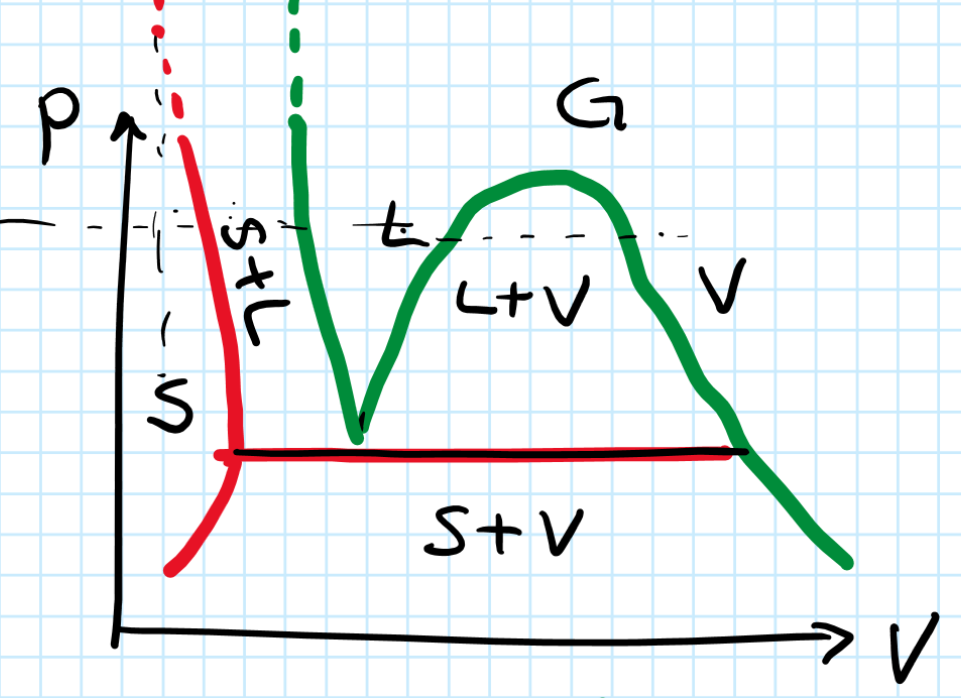
\includegraphics[width=7cm]{images/Grafico_p_V_transizione_di_stato.png}
\end{figure}

\begin{figure}[!htb]
    \centering
    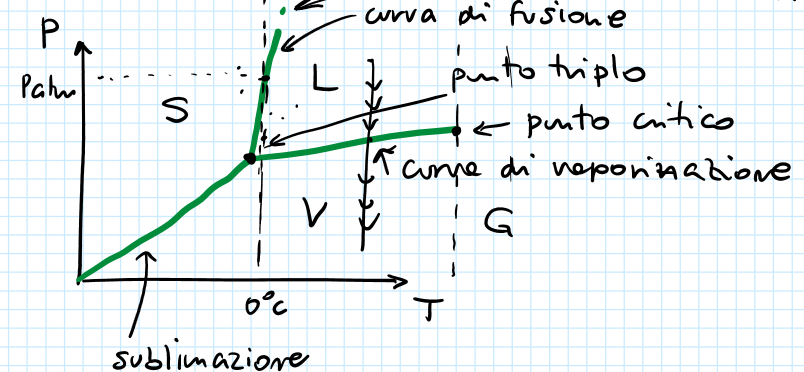
\includegraphics[width=11cm]{images/Grafico_p_T_transizione_stato.png}
\end{figure}


\subsection{Definizione di temperatura tramite gas}
L'esistenza del punto triplo ci permette di definire la temperatura in termini di una grandezza che possiamo misurare direttamente. 
\medskip

\noindent
A bassa pressione i gas tendono al regime di Gas ideale.\\
Se fissiamo il volume e le moli di gas possiamo definire $\theta$ in modo tale che $p=p_0(1+\al\theta)$, cio\`e poniamo 
\[\theta=\frac1\al\frac{p-p_0}{p_0}.\] 
Se imponiamo che l'acqua congeli per $\theta=0$ e evapori per $\theta=100$ allora ricaviamo $1/\al=273.15$. Notiamo inoltre\footnote{l'addizione di $\al\ii$ corrisponde alla traslazione che trasforma gradi Celsius in gradi Kelvin.}
\[\frac{p_2}{p_1}=\frac{\al\ii+\theta_2}{\al\ii +\theta_1}=\frac{\theta_2'}{\theta_1'}.\]
Possiamo dunque definire la temperatura (in Kelvin) come
\[T=\lim_{p^{(PT)}\to 0}273.16 \frac{p}{p^{(PT)}}\]
dove $p^{(PT)}$ \`e la pressione del gas nel termometro quando questo sistema \`e in equilibrio con il sistema di punto triplo con l'acqua. Il limite corrisponde a prendere gas sempre pi\`u rarefatti, cio\`e a lavorare nel limite dei gas perfetti dove vale la proporzionalit\`a sopra.
\medskip

\noindent Sfruttando questa definizione possiamo costruire un termometro a gas come in figura

\begin{figure}[!htb]
    \centering
    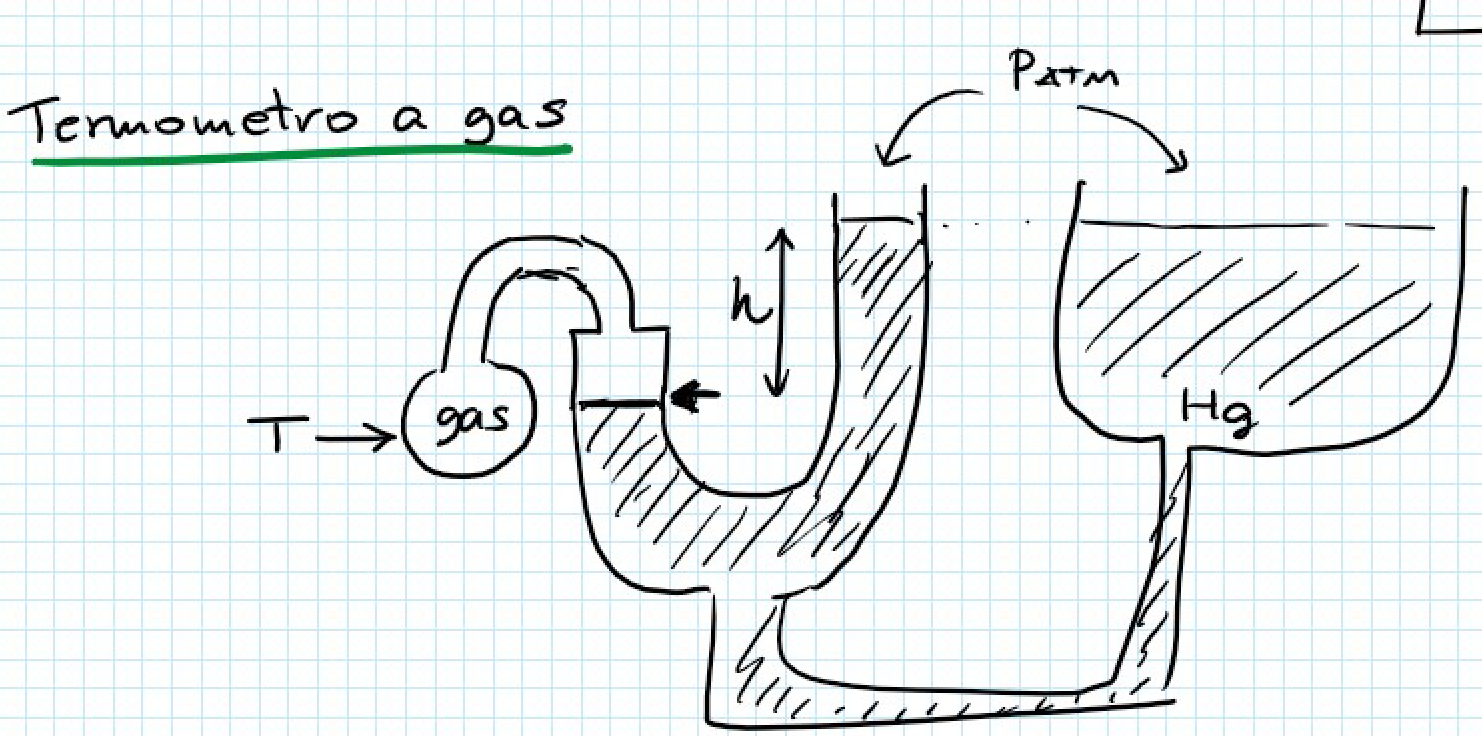
\includegraphics[width=11cm]{images/Termometro_a_gas.png}
\end{figure}


\noindent Quando il gas \`e alla temperatura che vogliamo misurare, misuriamo la differenza di altezza tra il livello a contatto con il gas e il livello di controllo posto a pressione atmosferica. 
Questa differenza \`e proporzionale alla differenza di pressione e questo ci permette di ricavare la temperatura se la fissiamo per quando \`e nel punto critico.




\section{Calore latente}
Consideriamo nuovamente il caso di due fasi (liquido e vapore). Osserviamo che fissata una temperatura, la pressione alla quale avviene la transizione di fase ne \`e una funzione. Segue che anche $V$ \`e una funzione di $T$.
\begin{remark}
Osserviamo che $dn_L=-dn_V$, quindi
\[\ppb VUT=\frac{u_V-u_L}{v_V-v_L}.\]
\end{remark}
\begin{proof}
Segue ricordando che $V=n_L v_L(T)+n_Vv_V(T)$ (e similmente per $U$) e che per le transizioni di fase $T$ \`e costante.
\end{proof}

\noindent
Per il primo principio
\[\delta Q=dU+pdV=dn_V(u_L-u_L+p(v_V-v_L)),\]
questo motiva la seguente
\begin{definition}[Calore latente]
Definiamo il \textbf{calore latente (molare) di vaporizzazione} come
\[\la=\frac{\delta Q}{dn_V}=u_V-u_L+p(v_V-v_L).\]
\end{definition}

\begin{proposition}[Equazione di Clapeyron]\label{EquazioneClapeyron}
Sulla transizione di fase
\[\dd Tp=\frac\la{T(v_V-v_L)}\]
\end{proposition}
\begin{proof}
Sviluppiamo $TdS$:
\[TdS=\under{=nc_V}{T\ppb TSVdT}+T\ppb VSTdV.\]
Applicando la relazione di Maxwell (\ref{RelazioniMaxwell}) data da $\ppb VST=\ppb TpV$ troviamo
\[TdS=nc_VdT+T\ppb TpVdV.\]
Combinando questo con $dU=TdS-pdV$ ricaviamo
\[dU=nc_VdT+\pa{T\ppb TpV-p}dV,\]
cio\`e
\[\ppb VUT=T\ppb TpV-p.\]
Ricordiamo ora che $\ppb VUT=\frac{u_V-u_L}{v_V-v_L}$, da cui
\[\frac\la{v_V-v_L}=T\ppb TpV,\]
che \`e la tesi se osserviamo che $\ppb TpV=\dd Tp$.
\end{proof}
\begin{remark}[Equazione di Clausius-Clapeyron]
Se $v_V\gg v_L$ allora per gas ideali
\[\dd Tp=\frac\la{RT^2}p\leadsto p\propto e^{-\la/RT}.\]
\end{remark}






















%\part{Relativit\`a speciale}

%\part{Basi di meccanica quantistica}


\appendix
\chapter{Richiami matematici}
\section{Derivate parziali e Jacobiane}
Da una relazione $f(x,y,z)=0$ possiamo ricavare $x=x(y,z)$ e $y=y(x,z)$.\\
Possiamo dunque sviluppare i differenziali
\begin{align*}
dx=&\ppb yxzdy+\ppb zxydz\\
dy=&\ppb xyzdx+\ppb zyxdz.
\end{align*}

\begin{proposition}[Propriet\`a delle derivate parziali]\label{ProprietaDerivateParziali}
Valgono le seguenti propriet\`a, dette \textbf{dell'inversa} e \textbf{ciclicit\`a} rispettivamente:
\[\ppb yxz=\pa{\ppb xyz}\ii,\qquad \ppb yxz\ppb zyx\ppb xzy=-1.\]
\end{proposition}
\begin{proof}
Considerando le espressioni date sopra e sostituiendo $dy$ dentro lo sviluppo di $dx$ ricaviamo l'equazione
\[\pa{1-\ppb yxz\ppb xyz}dx=\pa{\ppb yxz\ppb zyx+\ppb zxy}dz.\]
Se fissiamo $z$ il membro di sinistra non cambia, mentre quello di destra risulta nullo ($dz=0$). Poich\'e questo \`e vero anche per $dx\neq 0$ necessariamente ricaviamo
\[1=\ppb yxz\ppb xyz\]
che \`e la propriet\`a dell'inversa.\medskip

\noindent Avendo mostrato questo ricaviamo che il membro di sinistra \`e sempre nullo, anche per $dz\neq 0$, quindi segue l'equazione
\[\ppb yxz\ppb zyx+\ppb zxy=0,\]
la quale corrisponde alla propriet\`a di ciclicit\`a.
\end{proof}

\noindent Consideriamo le seguenti relazioni
\[\begin{cases}
x=x(u,v)\\
y=y(u,v)
\end{cases}.\]
Poniamo
\[\pp{(u,v)}{(x,y)}=det{\mat{\displaystyle\pp ux &\displaystyle\pp vx\\\\ \displaystyle\pp uy & \displaystyle\pp vy}}.\]
\begin{remark}[Jacobiane notevoli]\label{JacobianeNotevoli}
Si ha che
\[\pp{(x,y)}{(x,y)}=1,\quad \pp{(u,v)}{(x,x)}=0,\quad \pp{(u,v)}{(x,y)}=-\pp{(u,v)}{(y,x)}=\pp{(u,v)}{(-x,y)}.\]
Inoltre
\[\pp{(u,y)}{(x,y)}=\ppb uxy,\quad \pp{(u,v)}{(x,u)}=\pp{(r,s)}{(x,u)}\pp{(u,v)}{(r,s)},\quad \pp{(u,v)}{(x,y)}=\pa{\pp{(x,y)}{(u,v)}}\ii.\]
\end{remark}

\section{Differenziali esatti}
Ricordiamo che una forma $\sum A_i dx_i$ \`e chiusa quando per ogni coppia $i,j$
\[\pp {x_i}{A_j}=\pp{x_j}{A_i}.\]
Se il dominio \`e semplicemente connesso allora questa condizione caratterizza anche le forme esatte.

\begin{proposition}[Esattezza tramite Pfaff]\label{EsattezzaPfaff}
Sia $\sum_i A_idx_i$ una forma. Se l'equazione di Pfaff
\[\sum_i A_idx_i=0\]
\`e integrabile\footnote{cio\`e i punti che la verificano sono descrivibili tramite una equazione $F(x_1,\cdots, x_n)=cost.$} allora la forma \`e chiusa ed esiste $u(x_1,\cdots, x_n)$ tale che $\sum uA_i dx_i$ \`e esatta.
\end{proposition}
\begin{proof}
Sia $\cpa{F=0}$ l'equazione del luogo dove vale l'equazione Pfaff. Segue che
\[dF=\sum_i\pp{x_i}F dx_i=0=\sum_i A_idx_i,\]
esiste dunque $u$ tale che
\[\pp{x_i}F=u(x_1,\cdots, x_n)A_i,\]
da cui derivando
\[\pp{x_i}{}(uA_j)=\pp{x_i\del x_j}{^2F}=\pp{x_j}{}(uA_i),\]
cio\`e $\sum_i uA_idx_i$ \`e chiusa.
\end{proof}

\begin{fact}[Condizione di integrabilit\`a]
Se per ogni terna $i,\ j,\ k$ di indici distinti vale
\[A_k\pa{\pp {x_i}{A_j}-\pp {x_j}{A_i}}+A_j\pa{\pp {x_k}{A_i}-\pp {x_i}{A_k}}+A_i\pa{\pp {x_j}{A_k}-\pp {x_k}{A_j}}=0\]
allora $\sum A_i dx_i=0$ \`e integrabile.
\end{fact}

\begin{remark}\label{IntegrabilitaPuntiRaggiungibili}
Un sistema \`e integrabile se nell'intorno di un punto $P$ esistono infiniti punti non raggiungibili tramite percorsi su cui vale $\sum_i A_idx_i=0$ (ipersuperficie ha dimensione minore dello spazio ambiente).\medskip

\noindent
Segue che se posso raggiungere ogni punto rispettando l'equazione allora non avevamo integrabilit\`a
\end{remark}


\begin{example}
Consideriamo l'equazione $ydx+dy+dz=0$ e passiamo da $(0,0,0)$ a $(a,b,c)$:
\begin{itemize}
\item Variamo solo la $x$ ($dy=dz=0$). Poich\'e $y=0$ e non cambia l'equazione \`e rispettata e passiamo da $(0,0,0)$ a $(x_0,0,0)$ per un qualsiasi $x_0$.
\item Fissiamo $x=x_0$ ($dx=0$) e muoviamoci in modo tale che $dy=dz$ (lungo una diagonale) e cos\`i passiamo da $(x_0,0,0)$ a $(x_0,b,-b)$.
\item Fissiamo $y=b$ ($dy=0$) e muoviamoci in modo che $dz=-bdx$. Passiamo da $(x_0+(a-x_0),b,-b+(a-x_0)(-b))$. Se avevamo scelto $x_0$ in modo tale che $-b+(a-x_0)(-b)=c$ allora abbiamo finito.
\end{itemize}
\end{example}




\section{Trasformazione di Legendre}
Sia $F(x,y)$ con $dF=udx+vdy$\footnote{cio\`e $u=\ppb xFy$ e $v=\ppb yFx$.} e supponiamo di voler riformulare l'espressione in termini di $u$ e $y$. Definiamo 
\[G(u,y)=F-ux\]
e notiamo che
\[dG=dF-udx-xdu=\cancel{udx}+vdy-\cancel{udx}-xdu=vdy-xdu,\]
cio\`e $G$ effettivamente dipende esplicitamente solo da $u$ e $y$.

%\part*{Formulario}
%\include{Riconoscimenti.tex}

\end{document}